% 图 3.5 3d6 组态：(a) 高自旋 S=2 (b) 低自旋 S=0（八面体场 t2g/eg）
\documentclass[tikz,border=5pt]{standalone}
\usetikzlibrary{arrows.meta}
\usepackage{amsmath}
\usepackage{bm}
\usepackage{fontspec}
\setmainfont{Times New Roman}
\begin{document}
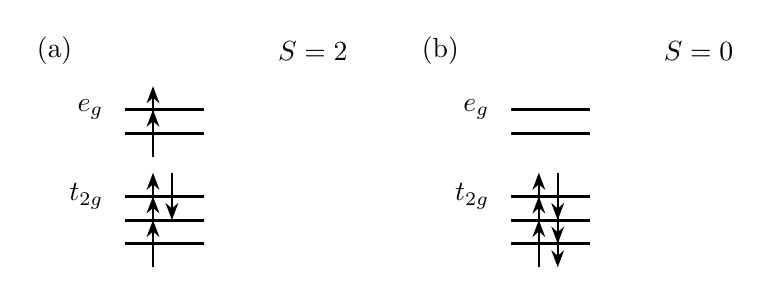
\begin{tikzpicture}[line width=0.8pt,>=Stealth]
% 电子箭头：\el{x}{能级y}{+1上 / -1下}
\newcommand{\el}[3]{
  \ifnum#3>0 \draw[->,line width=0.7] (#1,#2-0.30) -- (#1,#2+0.30);
  \else      \draw[->,line width=0.7] (#1,#2+0.30) -- (#1,#2-0.30);
  \fi}
\newcommand{\lev}[2]{\draw[line width=1.1] (#1,#2) -- (#1+1.0,#2);}
% ---------- (a) 高自旋 ----------
\begin{scope}
\node at (-0.2,2.95) {(a)};
\node[anchor=east] at (3.65,2.95) {$S=2$};
% e_g（上，两条单占据）
\node[anchor=east] at (0.55,2.20) {$e_g$};
\lev{0.70}{2.20} \el{1.05}{2.20}{1}
\lev{0.70}{1.90} \el{1.05}{1.90}{1}
% t_2g（下：一对 + 两个单占据）
\node[anchor=east] at (0.55,1.10) {$t_{2g}$};
\lev{0.70}{1.10} \el{1.05}{1.10}{1} \el{1.29}{1.10}{-1}
\lev{0.70}{0.80} \el{1.05}{0.80}{1}
\lev{0.70}{0.50} \el{1.05}{0.50}{1}
\end{scope}
% ---------- (b) 低自旋 ----------
\begin{scope}[shift={(4.9,0)}]
\node at (-0.2,2.95) {(b)};
\node[anchor=east] at (3.65,2.95) {$S=0$};
% e_g（上，空）
\node[anchor=east] at (0.55,2.20) {$e_g$};
\lev{0.70}{2.20}
\lev{0.70}{1.90}
% t_2g（下，三对）
\node[anchor=east] at (0.55,1.10) {$t_{2g}$};
\lev{0.70}{1.10} \el{1.05}{1.10}{1} \el{1.29}{1.10}{-1}
\lev{0.70}{0.80} \el{1.05}{0.80}{1} \el{1.29}{0.80}{-1}
\lev{0.70}{0.50} \el{1.05}{0.50}{1} \el{1.29}{0.50}{-1}
\end{scope}
\end{tikzpicture}
\end{document}
